% ============================================================
\chapter{\'Equation de Transport}
\label{ch:transport}
% ============================================================

Imaginez un polluant d\'evers\'e dans une rivi\`ere. Si le courant est
uniforme et qu'il n'y a ni diffusion ni r\'eaction chimique, le polluant se
d\'eplace simplement avec le fluide, comme un passager dans un train. C'est
l'\'equation de transport --- la plus simple de toutes les EDP, mais aussi
la plus fondamentale, car elle contient en germe la m\'ethode des
caract\'eristiques, qui sera notre outil principal pour toutes les \'equations
du premier ordre.

% ------------------------------------------------------------
\section{Introduction et motivation physique}
% ------------------------------------------------------------

L'\'equation de transport est la plus simple des EDP. Elle mod\'elise le
d\'eplacement d'une quantit\'e (concentration, densit\'e, polluant) transport\'ee
par un champ de vitesse sans diffusion ni r\'eaction.

\begin{intuition}
Imaginez un colorant inject\'e dans une rivi\`ere \`a courant uniforme.
Le colorant est emport\'e sans se m\'elanger~: sa concentration se d\'eplace
rigidement \`a la vitesse du courant. C'est exactement ce que d\'ecrit
l'\'equation de transport.
\end{intuition}

\section{\'Equation de transport \`a coefficients constants}

\subsection{Le probl\`eme de Cauchy}

\begin{definition}[\'Equation de transport homog\`ene]
L'\textbf{\'equation de transport} \`a vitesse constante $c \in \R$ est~:
\begin{equation}\label{eq:transport_homogene}
    \begin{cases}
        u_t + c\, u_x = 0, & x \in \R,\; t > 0,\\
        u(x,0) = u_0(x), & x \in \R.
    \end{cases}
\end{equation}
\end{definition}

\begin{theoreme}[Solution du probl\`eme de Cauchy]
Si $u_0 \in C^1(\R)$, alors le probl\`eme \eqref{eq:transport_homogene}
admet une unique solution $u \in C^1(\R \times [0,+\infty))$ donn\'ee par~:
\begin{equation}\label{eq:transport_solution}
    \boxed{u(x,t) = u_0(x - ct).}
\end{equation}
\end{theoreme}

\begin{proof}
\textbf{M\'ethode des caract\'eristiques.} Cherchons les courbes
$(x(t), t)$ dans le plan $(x,t)$ le long desquelles la solution $u$
est constante. Si $u$ est solution, posons $z(t) = u(x(t), t)$. Alors~:
\[
    z'(t) = u_t(x(t),t) + x'(t)\, u_x(x(t),t).
\]
Pour que $z'(t) = 0$ (solution constante le long de la courbe), il suffit
de choisir $x'(t) = c$, ce qui donne les \textbf{caract\'eristiques}~:
\[
    x(t) = x_0 + ct, \quad x_0 \in \R.
\]
Le long de chaque caract\'eristique, $u(x(t),t) = u(x_0, 0) = u_0(x_0)$.
En exprimant $x_0 = x - ct$, on obtient $u(x,t) = u_0(x-ct)$.

\textbf{V\'erification.} Si $u_0 \in C^1$, alors $u(x,t) = u_0(x-ct)$
est bien $C^1$ et~:
\[
    u_t = -c\, u_0'(x-ct), \quad u_x = u_0'(x-ct),
\]
donc $u_t + c\, u_x = 0$ et $u(x,0) = u_0(x)$.

\textbf{Unicit\'e.} Si $v$ est une autre solution $C^1$, alors
$w = u - v$ satisfait $w_t + c\, w_x = 0$ avec $w(x,0) = 0$. Le long
de toute caract\'eristique, $w$ est constante \'egale \`a $0$, donc $w \equiv 0$.
\end{proof}

\begin{center}
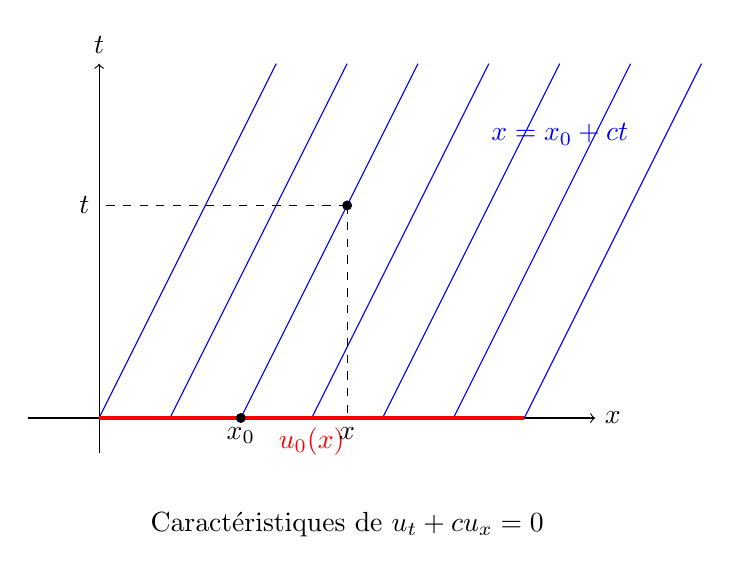
\begin{tikzpicture}[scale=0.9]
    \draw[->] (-1,0) -- (7,0) node[right] {$x$};
    \draw[->] (0,-0.5) -- (0,5) node[above] {$t$};
    % Caractéristiques
    \foreach \x in {0,1,2,3,4,5,6}{
        \draw[blue, thin] (\x,0) -- (\x+2.5, 5);
    }
    \node[blue] at (6.5, 4) {$x = x_0 + ct$};
    % Condition initiale
    \draw[very thick, red] (0,0) -- (6,0);
    \node[red, below] at (3,0) {$u_0(x)$};
    % Point
    \fill (2,0) circle (2pt) node[below] {$x_0$};
    \fill (3.5,3) circle (2pt);
    \draw[dashed] (3.5,3) -- (3.5,0) node[below] {$x$};
    \draw[dashed] (3.5,3) -- (0,3) node[left] {$t$};
    \node at (3.5, -1.5) {Caract\'eristiques de $u_t + cu_x = 0$};
\end{tikzpicture}
\end{center}

\begin{formules}[title=\textbf{\'Equation de transport --- formules cl\'es}]
\begin{itemize}
    \item Solution~: $u(x,t) = u_0(x - ct)$ (onde progressive).
    \item Caract\'eristiques~: droites $x - ct = \mathrm{cste}$.
    \item La solution se propage \`a vitesse $c$ sans d\'eformation.
\end{itemize}
\end{formules}

\subsection{\'Equation non homog\`ene}

\begin{theoreme}[Transport avec terme source]
Le probl\`eme~:
\begin{equation}\label{eq:transport_source}
    \begin{cases}
        u_t + c\, u_x = f(x,t), & x \in \R,\; t > 0,\\
        u(x,0) = u_0(x),
    \end{cases}
\end{equation}
admet pour solution~:
\begin{equation}\label{eq:transport_source_sol}
    u(x,t) = u_0(x-ct) + \int_0^t f(x - c(t-s), s)\, ds.
\end{equation}
\end{theoreme}

\begin{proof}
Le long de la caract\'eristique $x(s) = x - c(t-s)$, on a~:
\[
    \frac{d}{ds}u(x(s),s) = u_t + c\, u_x = f(x(s),s).
\]
En int\'egrant de $s=0$ \`a $s=t$~:
\[
    u(x,t) - u(x-ct, 0) = \int_0^t f(x - c(t-s), s)\, ds.
\]
\end{proof}

\section{M\'ethode des caract\'eristiques --- cas g\'en\'eral}

\subsection{EDP du premier ordre quasi-lin\'eaire}

Consid\'erons l'EDP g\'en\'erale du premier ordre~:
\begin{equation}\label{eq:quasi_lineaire}
    a(x,y,u)\, u_x + b(x,y,u)\, u_y = c(x,y,u).
\end{equation}

\begin{definition}[\'Equations caract\'eristiques]
Les \textbf{\'equations caract\'eristiques} associ\'ees \`a
\eqref{eq:quasi_lineaire} forment le syst\`eme d'EDO~:
\begin{equation}\label{eq:systeme_caract}
    \frac{dx}{a(x,y,u)} = \frac{dy}{b(x,y,u)} = \frac{du}{c(x,y,u)}.
\end{equation}
Ou de mani\`ere \'equivalente, en param\'etrant par $s$~:
\[
    \frac{dx}{ds} = a, \quad \frac{dy}{ds} = b, \quad \frac{du}{ds} = c.
\]
\end{definition}

\begin{theoreme}[Existence locale]
Soit $\Gamma$ une courbe initiale param\'etr\'ee par
$(x_0(\tau), y_0(\tau), u_0(\tau))$ telle que~:
\[
    \frac{\partial(x,y)}{\partial(s,\tau)}\bigg|_{s=0}
    = a\, y_0'(\tau) - b\, x_0'(\tau) \neq 0
    \quad \text{(condition de transversalit\'e)}.
\]
Alors il existe localement une unique solution $u(x,y)$ au voisinage
de $\Gamma$.
\end{theoreme}

\begin{attention}[title=\textbf{Condition de transversalit\'e}]
Si la courbe initiale est tangente aux caract\'eristiques en un point,
la m\'ethode \'echoue~: soit il n'y a pas de solution, soit il y en a
une infinit\'e. C'est analogue au probl\`eme de Cauchy pour les EDO quand
la condition initiale est pos\'ee en un point singulier.
\end{attention}

\begin{exemple}[EDP lin\'eaire \`a coefficients variables]
R\'esoudre~:
\[
    x\, u_x + y\, u_y = u, \quad u(x,1) = g(x).
\]
Les \'equations caract\'eristiques sont~:
\[
    \frac{dx}{x} = \frac{dy}{y} = \frac{du}{u}.
\]
De $\frac{dx}{x} = \frac{dy}{y}$, on obtient $\frac{x}{y} = C_1$
(constante). De $\frac{dy}{y} = \frac{du}{u}$, on obtient
$\frac{u}{y} = C_2$. Donc la solution g\'en\'erale est~:
\[
    u = y\, \Phi\!\left(\frac{x}{y}\right)
\]
pour une fonction arbitraire $\Phi$. La condition initiale $u(x,1) = g(x)$
donne $\Phi(x) = g(x)$, d'o\`u~:
\[
    u(x,y) = y\, g\!\left(\frac{x}{y}\right).
\]
\end{exemple}

\subsection{Cas non lin\'eaire~: \'equation de Burgers}

\begin{definition}[\'Equation de Burgers inviscide]
L'\textbf{\'equation de Burgers} est l'EDP non lin\'eaire~:
\begin{equation}\label{eq:burgers}
    u_t + u\, u_x = 0, \quad u(x,0) = u_0(x).
\end{equation}
\end{definition}

\begin{theoreme}[Solution implicite de Burgers]
Les caract\'eristiques de \eqref{eq:burgers} sont les droites~:
\[
    x = x_0 + u_0(x_0)\, t.
\]
Le long de chaque caract\'eristique, $u$ est constante~: $u = u_0(x_0)$.
La solution est d\'efinie implicitement par~:
\begin{equation}\label{eq:burgers_implicite}
    u(x,t) = u_0(x - u(x,t)\, t).
\end{equation}
\end{theoreme}

\begin{proof}
Les \'equations caract\'eristiques sont~:
\[
    \frac{dx}{ds} = u, \quad \frac{dt}{ds} = 1, \quad \frac{du}{ds} = 0.
\]
Donc $u$ est constante le long des caract\'eristiques, et $x(t) = x_0 + u_0(x_0)\, t$.
\end{proof}

\subsection{Formation de chocs}

\begin{theoreme}[Temps de formation du choc]
Si $u_0 \in C^1(\R)$ et $u_0'$ admet un minimum n\'egatif, alors les
caract\'eristiques se croisent au temps~:
\begin{equation}\label{eq:temps_choc}
    t^* = \frac{-1}{\min_{x \in \R} u_0'(x)} > 0.
\end{equation}
Pour $t < t^*$, la solution est $C^1$. Pour $t \geq t^*$, il se forme
un \textbf{choc} (discontinuit\'e).
\end{theoreme}

\begin{proof}
Deux caract\'eristiques issues de $x_0$ et $x_1 > x_0$ se croisent si~:
\[
    x_0 + u_0(x_0)\, t = x_1 + u_0(x_1)\, t,
\]
soit $t = \frac{x_1 - x_0}{u_0(x_0) - u_0(x_1)} = \frac{-1}{(u_0(x_1)-u_0(x_0))/(x_1-x_0)}$.
En passant \`a la limite $x_1 \to x_0$, le premier croisement a lieu \`a
$t^* = -1/\min u_0'$.
\end{proof}

\begin{center}
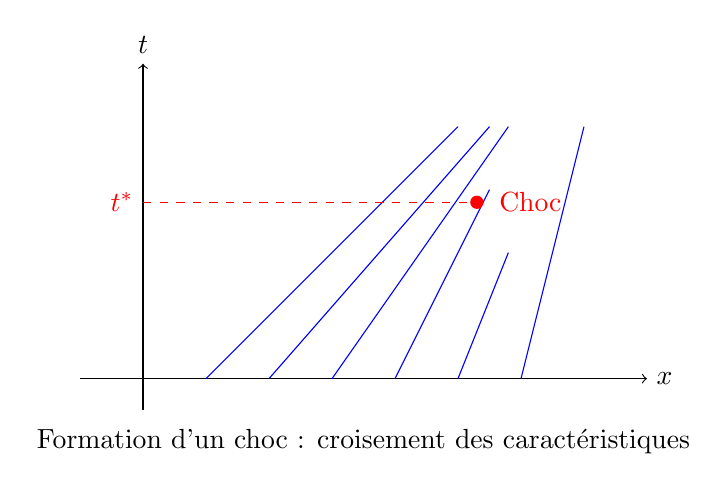
\begin{tikzpicture}[scale=0.8]
    \draw[->] (-1,0) -- (8,0) node[right] {$x$};
    \draw[->] (0,-0.5) -- (0,5) node[above] {$t$};
    % Caractéristiques qui se croisent
    \draw[blue] (1,0) -- (5,4);
    \draw[blue] (2,0) -- (5.5,4);
    \draw[blue] (3,0) -- (5.8,4);
    \draw[blue] (4,0) -- (5.5,3);
    \draw[blue] (5,0) -- (5.8,2);
    \draw[blue] (6,0) -- (7, 4);
    % Croisement
    \fill[red] (5.3, 2.8) circle (3pt);
    \node[red, right] at (5.5, 2.8) {Choc};
    % Temps critique
    \draw[dashed, red] (0,2.8) -- (5.3,2.8);
    \node[red, left] at (0,2.8) {$t^*$};
    \node at (3.5, -1) {Formation d'un choc~: croisement des caract\'eristiques};
\end{tikzpicture}
\end{center}

\begin{exemple}[Choc pour Burgers]
Soit $u_0(x) = 1 - x$ pour $x \in [0,1]$, $u_0(x) = 1$ pour $x < 0$,
$u_0(x) = 0$ pour $x > 1$. Alors $\min u_0' = -1$ (sur $]0,1[$), donc
$t^* = 1$. Les caract\'eristiques issues de $[0,1]$ sont
$x = x_0 + (1-x_0)t$ et elles se croisent toutes au point $(1,1)$.
\end{exemple}

\section{Transport en dimension sup\'erieure}

\begin{definition}[\'Equation de transport en $\R^n$]
Soit $\vec{b} = (b_1, \ldots, b_n) \in \R^n$ un vecteur vitesse constant.
L'\'equation de transport s'\'ecrit~:
\begin{equation}\label{eq:transport_Rn}
    u_t + \vec{b} \cdot \nabla u = 0, \quad u(x,0) = u_0(x),
    \quad x \in \R^n.
\end{equation}
La solution est $u(x,t) = u_0(x - \vec{b}\, t)$.
\end{definition}

Pour un champ de vitesse variable $\vec{b}(x,t)$, l'\'equation
$u_t + \vec{b}(x,t) \cdot \nabla u = 0$ se r\'esout encore par les
caract\'eristiques, qui sont les solutions de~:
\[
    \frac{d\vec{X}}{dt} = \vec{b}(\vec{X}(t), t), \quad \vec{X}(0) = x_0.
\]

\section{Conservation et int\'egrales premi\`eres}

\begin{proposition}[Conservation des normes $L^p$]
Si $u$ est solution de $u_t + c\, u_x = 0$ avec $u_0 \in L^p(\R)$,
$1 \leq p \leq \infty$, alors~:
\[
    \norm{u(\cdot, t)}_{L^p(\R)} = \norm{u_0}_{L^p(\R)}
    \quad \forall t \geq 0.
\]
\end{proposition}

\begin{proof}
Pour $1 \leq p < \infty$, le changement de variable $y = x - ct$ donne~:
\[
    \int_\R \abs{u(x,t)}^p\, dx
    = \int_\R \abs{u_0(x-ct)}^p\, dx
    = \int_\R \abs{u_0(y)}^p\, dy.
\]
Le cas $p = \infty$ est imm\'ediat.
\end{proof}

\begin{theoreme}[Forme conservative et condition de Rankine-Hugoniot]
L'\'equation $u_t + (f(u))_x = 0$ (loi de conservation) admet des solutions
faibles discontinues. \`A travers une discontinuit\'e se propageant \`a la
vitesse $\sigma$, la condition de \textbf{Rankine-Hugoniot} s'\'ecrit~:
\begin{equation}\label{eq:rankine_hugoniot}
    \sigma\, [u] = [f(u)],
\end{equation}
o\`u $[u] = u^+ - u^-$ d\'esigne le saut.
\end{theoreme}

\section{Solutions faibles et entropie}

\begin{definition}[Solution faible]
Une fonction $u \in L^\infty(\R \times [0,\infty))$ est une \textbf{solution
faible} de $u_t + (f(u))_x = 0$ avec donn\'ee initiale $u_0$ si~:
\[
    \int_0^\infty \int_\R \bigl[u\, \varphi_t + f(u)\, \varphi_x\bigr]\, dx\, dt
    + \int_\R u_0(x)\, \varphi(x,0)\, dx = 0
\]
pour toute $\varphi \in C_c^\infty(\R \times [0,\infty))$.
\end{definition}

\begin{attention}[title=\textbf{Non-unicit\'e des solutions faibles}]
Les solutions faibles ne sont en g\'en\'eral pas uniques~! Il faut
imposer une \textbf{condition d'entropie} pour s\'electionner la solution
physiquement admissible. La condition de Lax exige~:
\[
    f'(u^-) > \sigma > f'(u^+).
\]
\end{attention}

\section{Exercices}

\begin{exercice}
R\'esoudre $u_t + 3u_x = 0$, $u(x,0) = e^{-x^2}$. Tracer $u(x,t)$
pour $t = 0, 1, 2$.
\end{exercice}

\begin{exercice}
R\'esoudre $u_t + 2u_x = t\sin x$, $u(x,0) = 0$.
\end{exercice}

\begin{exercice}
R\'esoudre par les caract\'eristiques~:
$y\, u_x - x\, u_y = 0$, $u(x,0) = x^2$ pour $x > 0$.
Interpr\'eter g\'eom\'etriquement les caract\'eristiques.
\end{exercice}

\begin{exercice}
Soit l'\'equation de Burgers $u_t + u\, u_x = 0$ avec~:
\[
    u_0(x) = \begin{cases}
        1 & \text{si } x < 0,\\
        1 - x & \text{si } 0 \leq x \leq 1,\\
        0 & \text{si } x > 1.
    \end{cases}
\]
\begin{enumerate}
    \item Tracer les caract\'eristiques.
    \item D\'eterminer le temps $t^*$ de formation du choc.
    \item \'Ecrire la solution pour $0 < t < t^*$.
\end{enumerate}
\end{exercice}

\begin{exercice}
R\'esoudre l'\'equation de transport non lin\'eaire~:
$u_t + u^2 u_x = 0$, $u(x,0) = \frac{1}{1+x^2}$.
D\'eterminer le temps de formation du premier choc.
\end{exercice}

\begin{exercice}
Montrer que si $u$ est solution de $u_t + c\, u_x = 0$, alors
$E(t) = \frac{1}{2}\int_\R u^2(x,t)\, dx$ est conserv\'ee.
G\'en\'eraliser \`a $u_t + c(x)\, u_x = 0$ avec $c_x = 0$.
Que se passe-t-il si $c_x \neq 0$~?
\end{exercice}

\begin{exercice}[Ondes de rar\'efaction]
Consid\'erer l'\'equation de Burgers avec~:
\[
    u_0(x) = \begin{cases}
        0 & \text{si } x < 0,\\
        1 & \text{si } x > 0.
    \end{cases}
\]
\begin{enumerate}
    \item Montrer qu'il n'existe pas de solution classique pour $t > 0$.
    \item Construire une \textbf{onde de rar\'efaction} $u(x,t) = v(x/t)$
          solution faible continue.
    \item V\'erifier qu'une solution avec choc (de vitesse $\sigma = 1/2$)
          est aussi solution faible, mais ne satisfait pas la condition
          d'entropie de Lax.
\end{enumerate}
\end{exercice}
